\documentclass{article}
\usepackage{a4wide}
\usepackage{graphicx}
\setlength{\parindent}{0in}
\setlength{\parskip}{.1in}
\begin{document}

Many thanks to the anonymous reviewer and to the editor for identifying numerous
issues with the submission and providing helpful suggestions.  I have attempted
to address each of the issues in my revised submission, as described below.

\section*{Response to Anonymous Reviewer}

\begin{verbatim}
  It may be worth mentioning the origin of the name of the package - DVI files
  may be well known to LaTeX users but these are not mentioned until well into 
  the article, and are not explained at that point. An introduction of the 
  flow of .tex (source) -> .dvi (binary) -> .ps (render) may serve both new and
  experienced users well. For those not familiar with DVI files, the name may
  not seem related.
\end{verbatim}

\begin{verbatim}
  Nitpick: the {gridtext} and {ggtext} references could be reversed; these 
  render as "gridtext (Wilke and Wiernik, 2022b) and ggtext (Wilke and Wiernik, 
  2022a)" ('b' then 'a'). I notice the same ordering appears in the vignette.
\end{verbatim}

\begin{verbatim}
  "The gridtext and ggtext packages make it possible to change color within a
  character value, but they do not allow a mixture of plain text and 
  mathematical expressions." - it may be worthwhile explaining that these do 
  not support `<math>` tags which would otherwise be available to markdown 
  rendering. Whether this is a technical limitation or a lack of implementation 
  may be outside of the scope of this article, but that difference potentially 
  impacts the strength of the argument that "this cannot be done".
\end{verbatim}

\begin{verbatim}
  Nitpick: "The R graphics system can draw a character value across multiple
  lines, but only if explicit newlines are embedded in the character value
  (i.e., the line breaks are manual)." - I would challenge the use of the word
  "manual" here; `base::strwrap()` is able to achieve this, though as noted it
  embeds the linebreaks in the string; is not justified; and does not hyphenate.

  ```
  txt <- "We ‘move’ the original
  population’s mean to a new
  z_i and calculate the average
  fitness at that new mean
  phenotype of the population
  to get the adaptive landscape,
  W_i, then we combine the
  population mean and the average
  fitness to get the fitness function."
  plot(0:10, seq(0, 1, 0.1))
  text(2.5, 0.8, paste(strwrap(txt, width = 45), collapse = "\n"))
  ```
\end{verbatim}

\begin{verbatim}
  "Figure 1" - it may be helpful to describe the contents of this figure in the
  caption more clearly; viewing the article in monochrome, the significance of
  colour is lost.
\end{verbatim}

\begin{verbatim}
  "Figure 1: A plot with a text annotation that contains several typesetting
  challenges: in-line mathematical equations;" - should be
  "mathematical expressions"?
\end{verbatim}

\begin{verbatim}
  The 'supplementary materials' mentioned several times in the text appear to be
  incomplete; the `TeX` directory was not supplied. I was hoping to better
  understand the use of "local" LaTeX packages with the 'annotate-equations'
  example which references

  ```
  LaTeXpackage(name="annotate",
               preamble="\\usepackage{TeX/annotate-equations}")
  ```

  and it was unclear as to where 'TeX' refers. It seems this is a local, 
  relative directory, made clearer by a reference in the `purl` output

  ```
  schneiderLines <- readLines("TeX/schneider.tex")
  ```

  but this directory (and subsequently the .tex file) is omitted.
\end{verbatim}

\begin{verbatim}
  Some discussion regarding system-wide packages versus "local" package may be
  of benefit - can a seasoned LaTeX user leverage their suite of packages just 
  by adding the appropriate `\\usepackage{my-package}` preambles?
\end{verbatim}

\begin{verbatim}
  "Figure 12" and "Figure 13" - very hard to read in monochrome.
\end{verbatim}

\begin{verbatim}
  (Section 14: Discussion)
  It may be worthwhile adding some brief notes on the availability of packages
  for rendering LaTeX which don't have a stated goal of integrating into plots;
  e.g. {texPreview} and {latexpdf}.

  A link to the 'Literate Programming' section of the 'Reproducible Research'
  CRAN Task View

  https://cran.r-project.org/web/views/ReproducibleResearch.html

  may be of value here.
\end{verbatim}

\begin{verbatim}
  On Loading the package, user is presented with potentially cryptic details:
 
  ```
              TeX:  /Library/TeX/texbin/latex
            xetex:  XeTeX 3.141592653-2.6-0.999996 (TeX Live 2024)
           luatex:  This is LuaTeX, Version 1.18.0 (TeX Live 2024)
  luaotfload-tool:  3.28
  ```

  A header line explaining that this is the active configuration may be helpful,
  if this information is really required. Otherwise, offering a mechanism to
  purposefully expose it might be less confusing.
\end{verbatim}

\begin{verbatim}
  The article text notes:

  "The package start-up message reports on whether these are available."

  but I do not consider this a report on availability; merely a listing. Users
  unfamiliar with the *TeX family of software may find these names very 
  confusing.

  Given that this references a system installation of LaTeX, it raises the
  question of the dependence on {tinytex} - is that merely a fallback? Are there
  resolution strategies when packages are added to one or the other?
\end{verbatim}

\begin{verbatim}
  The article text notes:

  "An implicit limitation is that xdvir requires a TEX installation, though that
  is simplified through a dependency on the tinytex package (Xie, 2024)."

  but I have not tested the package on a system lacking a TeX installation.
\end{verbatim}

\begin{verbatim}
  There does not appear to be a package-wide help file (e.g. xdvir-package) 
  which would enable `?xdvir`. There _is_ a vignette which can be found with 
  `??xdvir` and this is a helpful addition.

  Help files are minimal; `?element_latex`, `?geom_latex`, `?LaTeXpackage` 
  provide no examples.
\end{verbatim}

\begin{verbatim}
  The mingling of R and LaTeX code is obviously a fine line to walk. I wonder if
  it would make sense to add some R wrappers which limit the amount of LaTeX 
  which needs to be written, for those less familiar with the document 
  structure, but are familiar with the expression syntax. For example, in this 
  block

  ```
  annotateEquations <-
      LaTeXpackage(name="annotate",
                   preamble="\\usepackage{TeX/annotate-equations}")
  registerPackage(annotateEquations)
  ```

  the `preamble` argument requires writing the LaTeX command `\\usepackage{}``
  with the remaining code all being R. A `source=` argument would
  enable not interleaving LaTeX code, but would expand to the `\\usepackage{}`
  line. This need not prevent additional preamble from being added.
\end{verbatim}

\begin{verbatim}
  It is not clear why `LaTeXpackage()` should not perform the 
  `registerPackage()` step itself; the article does not reference the 
  `annotateEquations` object after registration, merely the name "annotate" 
  provided there as an argument. Is that object useful outside of the 
  registration step?
\end{verbatim}

\begin{verbatim}
  Attempting to run one of the examples results, some issues are encountered

  ```
  library(xdvir)
  #>             TeX:  /Library/TeX/texbin/latex
  #>           xetex:  XeTeX 3.141592653-2.6-0.999996 (TeX Live 2024)
  #>          luatex:  This is LuaTeX, Version 1.18.0 (TeX Live 2024)
  #> luaotfload-tool:  3.28
  packageVersion("xdvir")
  #> [1] '0.1.2'
  library(ggplot2)
  packageVersion("ggplot2")
  #> [1] '3.5.1'

  tex <- r"(\huge $\Phi(z) = \frac{1}{\sqrt{2\pi}} \cdot e^{-\frac{z^2}{2}}$)"
  x <- seq(-4, 4, length.out=100)
  df <- data.frame(x=x, y=dnorm(x))

  gg <- ggplot(df) + geom_line(aes(x, y))

  gg +
    labs(title=paste("The Normal Distribution:", tex)) +
    theme(plot.title=element_latex())
  ```

\end{verbatim}

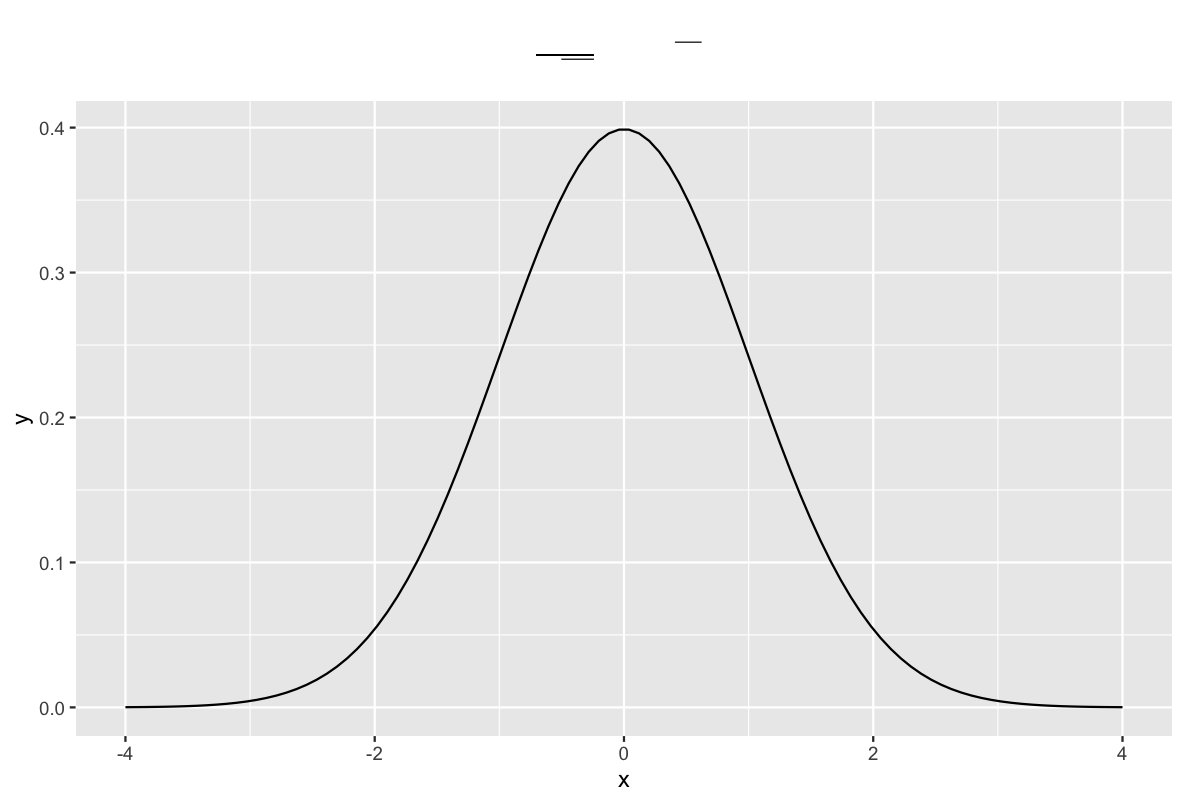
\includegraphics[width=\textwidth]{plot_issue.png}

\begin{verbatim}

  Created on 2025-04-06 with [reprex v2.1.1](https://reprex.tidyverse.org)
  ```

  (plot export attached). Test was performed on a Mac.
  
  I _am_ able to generate the rendered TeX with `plot.new(); grid.latex(tex)`.

  The package contains a `tests` directory, but it appears to not involve a 
  testing framework (e.g. {testthat}). Perhaps these tests are run manually? 
  The test code appears to only check that it runs without error, not that it 
  produces an expected result. I do not see any tests for {ggplot2} generated 
  figures, and no validation that this produces an expected result. Such a test
  may have caught the above issue.
\end{verbatim}

\section*{Response to Editor}

\begin{verbatim}
  The LaTeX \color{} command does not take a second argument. It simply changes
  the color from that point onwards. I think you mean \textcolor{}{}.
\end{verbatim}

Inappropriate uses of \verb|\color{}| have been changed to 
\verb|\textcolor{}|.

\begin{verbatim}
  In Figure 6, please use em-dashes (---) rather than hyphens (-).
\end{verbatim}

Hyphens have been replaced with em-dashes in Figure 6.

\begin{verbatim}
  You mix plain TeX commands within LaTeX environments. I suggest you replace 
  {\bf ..} with \textbf{..} and {\it ..} with \textit{..}. The results are not 
  identical.
\end{verbatim}

Instances of \verb|{\bf ...}| have been replaced with \verb|\textbf{...}|.

\begin{verbatim}
  In the discussion, it is perhaps worth including the ggtikz package.
\end{verbatim}

The \textbf{ggtikz} package 
is now mentioned in the Discussion, within the paragraph on 
the \textbf{tikzDevice} package.

\end{document}
